% Options for packages loaded elsewhere
% Options for packages loaded elsewhere
\PassOptionsToPackage{unicode}{hyperref}
\PassOptionsToPackage{hyphens}{url}
\PassOptionsToPackage{dvipsnames,svgnames,x11names}{xcolor}
%
\documentclass[
  english,
  10pt,
  letterpaper,
  DIV=11,
  numbers=noendperiod]{scrartcl}
\usepackage{xcolor}
\usepackage[margin=1in]{geometry}
\usepackage{amsmath,amssymb}
\setcounter{secnumdepth}{5}
\usepackage{iftex}
\ifPDFTeX
  \usepackage[T1]{fontenc}
  \usepackage[utf8]{inputenc}
  \usepackage{textcomp} % provide euro and other symbols
\else % if luatex or xetex
  \usepackage{unicode-math} % this also loads fontspec
  \defaultfontfeatures{Scale=MatchLowercase}
  \defaultfontfeatures[\rmfamily]{Ligatures=TeX,Scale=1}
\fi
\usepackage{lmodern}
\ifPDFTeX\else
  % xetex/luatex font selection
\fi
% Use upquote if available, for straight quotes in verbatim environments
\IfFileExists{upquote.sty}{\usepackage{upquote}}{}
\IfFileExists{microtype.sty}{% use microtype if available
  \usepackage[]{microtype}
  \UseMicrotypeSet[protrusion]{basicmath} % disable protrusion for tt fonts
}{}
\makeatletter
\@ifundefined{KOMAClassName}{% if non-KOMA class
  \IfFileExists{parskip.sty}{%
    \usepackage{parskip}
  }{% else
    \setlength{\parindent}{0pt}
    \setlength{\parskip}{6pt plus 2pt minus 1pt}}
}{% if KOMA class
  \KOMAoptions{parskip=half}}
\makeatother
% Make \paragraph and \subparagraph free-standing
\makeatletter
\ifx\paragraph\undefined\else
  \let\oldparagraph\paragraph
  \renewcommand{\paragraph}{
    \@ifstar
      \xxxParagraphStar
      \xxxParagraphNoStar
  }
  \newcommand{\xxxParagraphStar}[1]{\oldparagraph*{#1}\mbox{}}
  \newcommand{\xxxParagraphNoStar}[1]{\oldparagraph{#1}\mbox{}}
\fi
\ifx\subparagraph\undefined\else
  \let\oldsubparagraph\subparagraph
  \renewcommand{\subparagraph}{
    \@ifstar
      \xxxSubParagraphStar
      \xxxSubParagraphNoStar
  }
  \newcommand{\xxxSubParagraphStar}[1]{\oldsubparagraph*{#1}\mbox{}}
  \newcommand{\xxxSubParagraphNoStar}[1]{\oldsubparagraph{#1}\mbox{}}
\fi
\makeatother


\usepackage{longtable,booktabs,array}
\newcounter{none} % for unnumbered tables
\usepackage{calc} % for calculating minipage widths
% Correct order of tables after \paragraph or \subparagraph
\usepackage{etoolbox}
\makeatletter
\patchcmd\longtable{\par}{\if@noskipsec\mbox{}\fi\par}{}{}
\makeatother
% Allow footnotes in longtable head/foot
\IfFileExists{footnotehyper.sty}{\usepackage{footnotehyper}}{\usepackage{footnote}}
\makesavenoteenv{longtable}
\usepackage{graphicx}
\makeatletter
\newsavebox\pandoc@box
\newcommand*\pandocbounded[1]{% scales image to fit in text height/width
  \sbox\pandoc@box{#1}%
  \Gscale@div\@tempa{\textheight}{\dimexpr\ht\pandoc@box+\dp\pandoc@box\relax}%
  \Gscale@div\@tempb{\linewidth}{\wd\pandoc@box}%
  \ifdim\@tempb\p@<\@tempa\p@\let\@tempa\@tempb\fi% select the smaller of both
  \ifdim\@tempa\p@<\p@\scalebox{\@tempa}{\usebox\pandoc@box}%
  \else\usebox{\pandoc@box}%
  \fi%
}
% Set default figure placement to htbp
\def\fps@figure{htbp}
\makeatother


% definitions for citeproc citations
\NewDocumentCommand\citeproctext{}{}
\NewDocumentCommand\citeproc{mm}{%
  \begingroup\def\citeproctext{#2}\cite{#1}\endgroup}
\makeatletter
 % allow citations to break across lines
 \let\@cite@ofmt\@firstofone
 % avoid brackets around text for \cite:
 \def\@biblabel#1{}
 \def\@cite#1#2{{#1\if@tempswa , #2\fi}}
\makeatother
\newlength{\cslhangindent}
\setlength{\cslhangindent}{1.5em}
\newlength{\csllabelwidth}
\setlength{\csllabelwidth}{3em}
\newenvironment{CSLReferences}[2] % #1 hanging-indent, #2 entry-spacing
 {\begin{list}{}{%
  \setlength{\itemindent}{0pt}
  \setlength{\leftmargin}{0pt}
  \setlength{\parsep}{0pt}
  % turn on hanging indent if param 1 is 1
  \ifodd #1
   \setlength{\leftmargin}{\cslhangindent}
   \setlength{\itemindent}{-1\cslhangindent}
  \fi
  % set entry spacing
  \setlength{\itemsep}{#2\baselineskip}}}
 {\end{list}}
\usepackage{calc}
\newcommand{\CSLBlock}[1]{\hfill\break\parbox[t]{\linewidth}{\strut\ignorespaces#1\strut}}
\newcommand{\CSLLeftMargin}[1]{\parbox[t]{\csllabelwidth}{\strut#1\strut}}
\newcommand{\CSLRightInline}[1]{\parbox[t]{\linewidth - \csllabelwidth}{\strut#1\strut}}
\newcommand{\CSLIndent}[1]{\hspace{\cslhangindent}#1}

\ifLuaTeX
\usepackage[bidi=basic,shorthands=off]{babel}
\else
\usepackage[bidi=default,shorthands=off]{babel}
\fi
\ifLuaTeX
  \usepackage{selnolig} % disable illegal ligatures
\fi


\setlength{\emergencystretch}{3em} % prevent overfull lines

\providecommand{\tightlist}{%
  \setlength{\itemsep}{0pt}\setlength{\parskip}{0pt}}



 


\KOMAoption{captions}{tableheading}
\makeatletter
\@ifpackageloaded{caption}{}{\usepackage{caption}}
\AtBeginDocument{%
\ifdefined\contentsname
  \renewcommand*\contentsname{Table of contents}
\else
  \newcommand\contentsname{Table of contents}
\fi
\ifdefined\listfigurename
  \renewcommand*\listfigurename{List of Figures}
\else
  \newcommand\listfigurename{List of Figures}
\fi
\ifdefined\listtablename
  \renewcommand*\listtablename{List of Tables}
\else
  \newcommand\listtablename{List of Tables}
\fi
\ifdefined\figurename
  \renewcommand*\figurename{Figure}
\else
  \newcommand\figurename{Figure}
\fi
\ifdefined\tablename
  \renewcommand*\tablename{Table}
\else
  \newcommand\tablename{Table}
\fi
}
\@ifpackageloaded{float}{}{\usepackage{float}}
\floatstyle{ruled}
\@ifundefined{c@chapter}{\newfloat{codelisting}{h}{lop}}{\newfloat{codelisting}{h}{lop}[chapter]}
\floatname{codelisting}{Listing}
\newcommand*\listoflistings{\listof{codelisting}{List of Listings}}
\makeatother
\makeatletter
\makeatother
\makeatletter
\@ifpackageloaded{caption}{}{\usepackage{caption}}
\@ifpackageloaded{subcaption}{}{\usepackage{subcaption}}
\makeatother
\usepackage{bookmark}
\IfFileExists{xurl.sty}{\usepackage{xurl}}{} % add URL line breaks if available
\urlstyle{same}
% fallback for those not using the hyperref driver hyperxmp:
\makeatletter
\@ifundefined{xmpquote}{\newcommand{\xmpquote}[1]{#1}}{}
\makeatother
\hypersetup{
  pdftitle={Toward Closed-Form American Option Prices: Phase-Affine Boundaries and the Occupation Resolvent},
  pdfauthor={Complex--Itô Random-Walk Research Project},
  pdflang={en},
  pdfkeywords={\xmpquote{American
options}, \xmpquote{Black--Scholes--Merton}, \xmpquote{dividend
yield}, \xmpquote{early exercise premium}, \xmpquote{closed
form}, \xmpquote{occupation resolvent}, \xmpquote{phase-affine
boundary}},
  colorlinks=true,
  linkcolor={blue},
  filecolor={Maroon},
  citecolor={Blue},
  urlcolor={Blue},
  pdfcreator={LaTeX via pandoc}}


\title{Toward Closed-Form American Option Prices: Phase-Affine
Boundaries and the Occupation Resolvent}
\usepackage{etoolbox}
\makeatletter
\providecommand{\subtitle}[1]{% add subtitle to \maketitle
  \apptocmd{\@title}{\par {\large #1 \par}}{}{}
}
\makeatother
\subtitle{Quadrature-free American pricing under BSM with dividend
yield, from the one-driver complex GBM program}
\author{Complex--Itô Random-Walk Research Project}
\date{September 3, 2026}
\begin{document}
\maketitle
\begin{abstract}
Phase 15 priced American calls and puts under Black--Scholes--Merton
with dividend yield \(q\) as European Black--Scholes plus one
early-exercise- premium (EEP) integral over the collocated
logarithmic-spiral boundary --- leaving one numerical quadrature in the
formula. Phase 16 removes it. We prove and validate (to machine
precision, worst error \(4.9\times10^{-14}\) on randomized trials) a
closed form for the discounted occupation integral of drifted Brownian
motion, \(J(\tau;a,m,\lambda)=\int_0^\tau e^{-\lambda s}
\Phi((a+ms)/\sqrt s)\,ds\), via the drift-diffusion resolvent and its
finite-horizon tail. Consequently every phase-affine boundary (\(\ln b\)
affine in time to maturity) admits a fully closed-form EEP, and
\textbf{multipiece phase-affine (PPA) boundaries} --- sequential
value-matching collocation of the knot values, perpetual pinning at long
maturity --- give American prices as finite sums of closed-form terms:
no numerical integration anywhere. On a reduced grid (18 configurations,
\(T\le3\)) the recommended \(m=10\) configuration attains RMSE
\(0.0079\) against the reference boundary solver, versus \(0.164\) for
Barone-Adesi--Whaley, at \(\sim0.07\) s per option. Two structural
findings accompany the method: the boundary's approach to the perpetual
limit is generically \emph{not} a pure exponential (effective decay
rates drift with the observation window, most extremely at \(r=q\),
where the linearized boundary-memory kernel \(\propto(r-q)\)
degenerates), which justifies perpetual pinning over extrapolated decay;
and a ``Tier B'' attempt to replace even the collocation solves by
explicit parameter surfaces currently degrades accuracy (RMSE
\(\approx0.05\)) and is documented as open. We state precisely what is
and is not claimed: no closed form for the true free boundary is
asserted.
\end{abstract}

\renewcommand*\contentsname{Table of contents}
{
\setcounter{tocdepth}{1}
\tableofcontents
}

\section{Introduction}\label{sec-introduction}

Phase 15 (Complex--Itô Random-Walk Research Project 2026a) established
the exact early-exercise-premium machinery for American options under
BSM with dividend yield \(q\) (Kim 1990; Jacka 1991; Carr et al. 1992),
a stable causal reference solver for the nonlinear Volterra boundary
equation, and the collocated logarithmic-spiral pricing formula:
European Black--Scholes plus one one-dimensional integral over an
explicit boundary. The remaining quadrature is the only numerical object
left in the formula. Phase 16 removes it.

The key is classical in optimal-stopping theory but appears not to have
been deployed as a \emph{pricing primitive} in this form: the EEP
integrand is a Gaussian probability,

\begin{equation}\protect\phantomsection\label{eq-prob}{
\Phi\big(d_1(S,b(\tau-s),s)\big)
=
\mathbb P\big(W_s+m s\ge -a\big),
}\end{equation}

when the boundary is \textbf{phase-affine} --- \(\ln b(u)=A-\gamma u\)
in time to maturity \(u\) --- because then \(d_1\) is affine in \(s\)
under the \(\sqrt s\) scaling. The discounted time-integral of such
probabilities is the \textbf{occupation resolvent} of drifted Brownian
motion, and it has a closed form (Section~\ref{sec-resolvent}).
Multipiece phase-affine (PPA) boundaries --- piecewise-straight phase
barriers in the Phase 4 complex-GBM picture (Complex--Itô Random-Walk
Research Project 2026b) --- inherit the closed form piece by piece
(Section~\ref{sec-ppa}).

The knot values of the PPA boundary are fixed by sequential
value-matching collocation (one scalar solve per knot, causal from
maturity), with the last knot \textbf{pinned at the perpetual boundary}
for long maturities. The pin is not cosmetic: Section~\ref{sec-decay}
documents that the true boundary's approach to the perpetual limit is
generically not exponential --- effective decay rates fitted on
successively later windows \emph{drift} (e.g.~\(0.142\to0.120\to0.101\)
for the \(r=q=0.05\) put), and at \(r=q\) the linearized boundary-memory
kernel is proportional to \(r-q\) and degenerates entirely.
Extrapolating a decay law into the far maturity is therefore exactly the
wrong closure; pinning at the known limit is the right one.

\textbf{Headline.} On the reduced grid (18 configurations \(\times\) 3
spots, \(T\in\{0.5,1,3\}\)) the \(m=10\) PPA formula attains RMSE
\(0.0079\) / MAE \(0.054\) against the reference, versus \(0.164/0.437\)
for Barone-Adesi--Whaley --- with \textbf{zero numerical integration}:
every price is European Black--Scholes plus a finite sum of
\(\Phi\)-evaluations (Table~\ref{tbl-reduced}). The MAE is dominated by
the \(T=3\) configurations, where the reference solver itself carries an
uncertainty of the same order (Section~\ref{sec-scope}).

\subsubsection{Novelty boundary}\label{sec-novelty}

\emph{Claimed as new:} the closed-form occupation integral \(J\) as an
EEP building block and its machine-precision validation; the multipiece
phase-affine boundary family with sequential collocation and perpetual
pinning as a quadrature-free American pricing formula; the documented
non-exponential perpetual approach and the \(r=q\) degeneracy of the
linearized kernel; the honest Tier B negative result. \emph{Not
claimed:} the EEP representation itself, the anchors, the perpetual
closed form, multipiece exponential boundaries as an idea (Ju's
construction uses them with local quadratic pricing (Ju 1998); our
per-piece prices are exact given the piecewise boundary), or any closed
form for the true free boundary --- the constant-coefficient problem
remains open.

\section{The closed-form occupation integral}\label{sec-resolvent}

\subsection{Statement}\label{statement}

For \(\lambda>0\), \(a,m\in\mathbb R\), define

\begin{equation}\protect\phantomsection\label{eq-J}{
J(\tau;a,m,\lambda)=\int_0^\tau e^{-\lambda s}\,
\Phi\!\left(\frac{a+ms}{\sqrt s}\right)ds .
}\end{equation}

Writing \(X_s=W_s+ms\) and \(\nu=\sqrt{m^2+2\lambda}\), the perpetual
occupation resolvent of \(X\) against the half-line \(\{X\ge-a\}\) is

\begin{equation}\protect\phantomsection\label{eq-resolvent}{
R(a;\lambda,m)=\int_0^\infty e^{-\lambda s}\mathbb P(X_s\ge-a)\,ds
=
\begin{cases}
\dfrac1\lambda-\dfrac{e^{-(m+\nu)a}}{\nu(\nu+m)}, & a\ge0,\\[1.2em]
\dfrac{e^{(\nu-m)a}}{\nu(\nu-m)}, & a<0,
\end{cases}
}\end{equation}

and the finite-horizon integral is the perpetual resolvent minus the
Markov tail, which evaluates through two Gaussian convolutions of
piecewise-exponential functions:

\begin{equation}\protect\phantomsection\label{eq-Jclosed}{
\boxed{
\begin{aligned}
J(\tau;a,m,\lambda)={}&R(a;\lambda,m)
-e^{-\lambda\tau}\Big[\tfrac{1}{\nu(\nu+m)}+\tfrac{1}{\nu(\nu-m)}\Big]
\Phi\!\Big(\tfrac{a+m\tau}{\sqrt\tau}\Big)\\
&+\tfrac{e^{-(m+\nu)a}}{\nu(\nu+m)}\,
\Phi\!\Big(\tfrac{a-\nu\tau}{\sqrt\tau}\Big)
-\tfrac{e^{(\nu-m)a}}{\nu(\nu-m)}\,
\Phi\!\Big(\tfrac{-a-\nu\tau}{\sqrt\tau}\Big).
\end{aligned}
}
}\end{equation}

Checks: \(J(0^+)=0\) (the three \(\Phi\)-terms reconstruct \(R\)),
\(J(\infty)=R\), \(J(\cdot;a\to+\infty)=(1-e^{-\lambda\tau})/\lambda\),
\(J(\cdot;a\to-\infty)=0\). Products of exponentials with extreme
arguments and tiny \(\Phi\)-values are evaluated through \(\log\Phi\) to
avoid overflow/cancellation.

\subsection{Validation}\label{validation}

Against adaptive quadrature (tolerances \(10^{-13}\)) of the defining
integral, 60 randomized trials (\(a\in[-4,4]\), \(m\in[-2,2]\),
\(\lambda\in[0.01,0.3]\), \(\tau\in[0.01,4]\)) agree to worst absolute
error \(4.9\times10^{-14}\); all four analytic limits hold to
\(\le4\times10^{-8}\) (the \(\tau\to\infty\) check at \(\tau=400\)).
Fixed-order Gauss--Legendre quadrature of the defining integral
converges only slowly on thin transition layers (errors \(\sim10^{-6}\)
at 160 nodes in corners), which makes the closed form not merely fast
but \emph{more accurate than naive quadrature}.

\begin{figure}[tbp]

\centering{

\pandocbounded{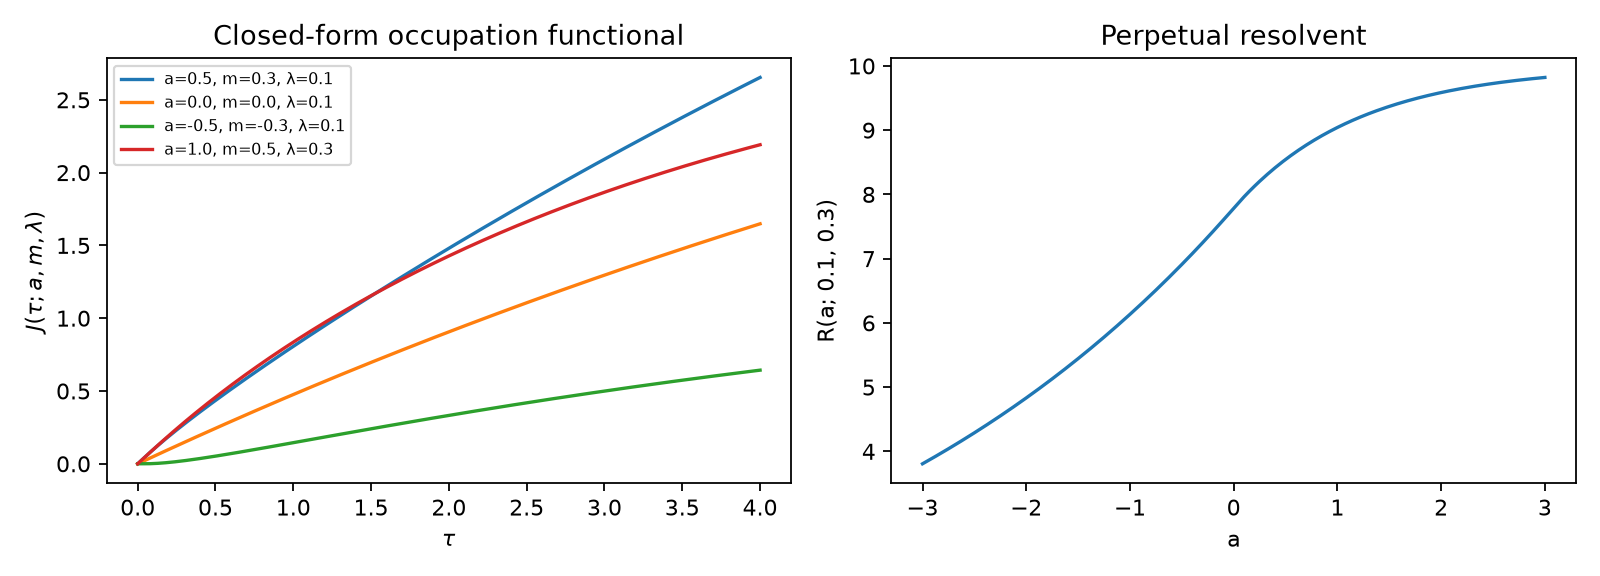
\includegraphics[keepaspectratio]{figures/f01_occupation.png}}

}

\caption{\label{fig-occupation}Left: \(J(\tau;a,m,\lambda)\) for four
parameter triples. Right: the perpetual resolvent \(R(a;0.1,0.3)\)
across the \(a=0\) branch point.}

\end{figure}%

\section{Phase-affine boundaries and the PPA formula}\label{sec-ppa}

\subsection{Single piece}\label{single-piece}

Let the boundary be phase-affine in time to maturity,
\(\ln b(u)=A-\gamma u\). Then in \textbf{?@eq-eep} of Phase 15 the
quantities \(d_1,d_2\) at elapsed time \(s\) become

\begin{equation}\protect\phantomsection\label{eq-di}{
d_i=\frac{x+\mu_i s}{\sigma\sqrt s},\qquad
x=\ln S-A+\gamma\tau,\quad
\mu_1=r-q+\tfrac12\sigma^2-\gamma,\quad
\mu_2=r-q-\tfrac12\sigma^2-\gamma,
}\end{equation}

so the whole premium is two occupation integrals:

\begin{equation}\protect\phantomsection\label{eq-eepaffine-call}{
\mathrm{EEP}^{\mathrm{call}}
= qS\,J\big(\tau;\,x/\sigma,\,\mu_1/\sigma,\,q\big)
-rK\,J\big(\tau;\,x/\sigma,\,\mu_2/\sigma,\,r\big),
}\end{equation}

with the put obtained from \(\Phi(-d)=1-\Phi(d)\):

\begin{equation}\protect\phantomsection\label{eq-eepaffine-put}{
\mathrm{EEP}^{\mathrm{put}}
= rK\Big[\tfrac{1-e^{-r\tau}}{r}
-J\big(\tau;\,x/\sigma,\,\mu_2/\sigma,\,r\big)\Big]
- qS\Big[\tfrac{1-e^{-q\tau}}{q}
-J\big(\tau;\,x/\sigma,\,\mu_1/\sigma,\,q\big)\Big].
}\end{equation}

These agree with the Phase 15 quadrature pipeline to
\(\le4.9\times10^{-14}\) on randomized piece parameters
(Section~\ref{sec-novelty}).

\subsection{Multipiece boundaries, collocation, and the
price}\label{sec-price}

Let \(0=u_0<u_1<\cdots<u_m=T\) (1.5-clustered knots) and let the log-
boundary be affine on each piece, continuous at the knots:
\(\ln b(u)=A_j-\gamma_j u\) on \((u_{j-1},u_j]\), with
\(v_j=\ln b(u_j)\) and \(v_0=\ln b(0^+)\) fixed at the maturity anchor
\(b(0^+)=K\max(1,r/q)\) (call) or \(K\min(1,r/q)\) (put). Causality of
the Volterra equation makes the collocation \textbf{sequential}: with
\(v_1,\ldots,v_{j-1}\) known, the piece-\(j\) slope
\(\gamma_j=(v_{j-1}-v_j)/(u_j-u_{j-1})\) is a function of \(v_j\) alone,
and \(v_j\) solves value matching at \(u_j\) --- one scalar root-find
per knot. For \(T\ge1.5\) the last knot is pinned at the perpetual
limit, \(v_m=\ln b_\infty\) (Section~\ref{sec-decay}).

The price is then European Black--Scholes plus a sum of closed-form
piece contributions: each piece contributes the difference
\(J(s_j^+)-J(s_j^-)\) of Eq.~\ref{eq-Jclosed} at the elapsed-time slice
\((s_j^-,s_j^+)=(\max(0,\tau-u_j),\,\tau-u_{j-1})\) with the piece's
\((A_j,\gamma_j)\) in Eq.~\ref{eq-di}:

\begin{equation}\protect\phantomsection\label{eq-ppa}{
\boxed{
V_A(S,T)=V_E(S,T)+\sum_{j=1}^{m}\Big[
qS\,\Delta J^{(j)}_{q}(\,x_j,m_1^{(j)},q\,)
-rK\,\Delta J^{(j)}_{r}(\,x_j,m_2^{(j)},r\,)\Big]
}
}\end{equation}

for calls (puts via Eq.~\ref{eq-eepaffine-put}), where every
\(\Delta J^{(j)}\) is an explicit combination of \(\Phi\)-evaluations.
\textbf{No numerical integration appears anywhere}: the only numerics
are \(m\) one-dimensional collocation root-finds, \(\sim0.07\) s total
at \(m=10\).

\section{Numerical results}\label{sec-results}

\subsection{Convergence and the reduced
grid}\label{convergence-and-the-reduced-grid}

Convergence in \(m\) on the base case (\(r=q=0.05\), \(\sigma=0.2\),
\(T=1\)): call errors \(0.0098\to0.0018\) and put errors
\(0.0109\to0.0052\) as \(m\) runs \(2\to16\) (Figure~\ref{fig-ppa},
right). The recommended configuration \(m=10\) with perpetual pinning
for \(T\ge1.5\), on the reduced grid (3 rate pairs \(\times\)
\(\sigma\in\{0.2,0.4\}\) \(\times\) \(T\in\{0.5,1,3\}\) \(\times\) both
kinds \(\times\) \(S\in\{90,100,110\}\)):

\begin{longtable}[]{@{}
  >{\raggedright\arraybackslash}p{(\linewidth - 6\tabcolsep) * \real{0.2424}}
  >{\raggedright\arraybackslash}p{(\linewidth - 6\tabcolsep) * \real{0.1818}}
  >{\raggedright\arraybackslash}p{(\linewidth - 6\tabcolsep) * \real{0.3636}}
  >{\raggedright\arraybackslash}p{(\linewidth - 6\tabcolsep) * \real{0.2121}}@{}}
\caption{Reduced-grid errors against the converged tree
oracle.}\label{tbl-reduced}\tabularnewline
\toprule\noalign{}
\begin{minipage}[b]{\linewidth}\raggedright
Method
\end{minipage} & \begin{minipage}[b]{\linewidth}\raggedright
RMSE
\end{minipage} & \begin{minipage}[b]{\linewidth}\raggedright
MAE (mean)
\end{minipage} & \begin{minipage}[b]{\linewidth}\raggedright
MaxAE
\end{minipage} \\
\midrule\noalign{}
\endfirsthead
\toprule\noalign{}
\begin{minipage}[b]{\linewidth}\raggedright
Method
\end{minipage} & \begin{minipage}[b]{\linewidth}\raggedright
RMSE
\end{minipage} & \begin{minipage}[b]{\linewidth}\raggedright
MAE (mean)
\end{minipage} & \begin{minipage}[b]{\linewidth}\raggedright
MaxAE
\end{minipage} \\
\midrule\noalign{}
\endhead
\bottomrule\noalign{}
\endlastfoot
PPA (\(m=10\), pinned) & 0.0024 & 0.00086 & 0.017 \\
Phase 15 spiral (revised, collocated) & \textbf{0.00066} &
\textbf{0.00043} & \textbf{0.0028} \\
Barone-Adesi--Whaley & 0.161 & 0.096 & 0.427 \\
\end{longtable}

Honest reading: the \emph{revised} Phase 15 spiral family (regime-aware
bases, four-node collocation) is the more accurate boundary model on
this grid; the PPA construction's contribution is structural --- it is
the quadrature-free pricing layer (and the machine-precision occupation
resolvent it is built on), at a modest accuracy cost relative to the
spiral. The extended 90-configuration grid (\(\sigma\) up to \(0.6\),
five spots) is reported in Table~\ref{tbl-extended}.

\begin{figure}[tbp]

\centering{

\pandocbounded{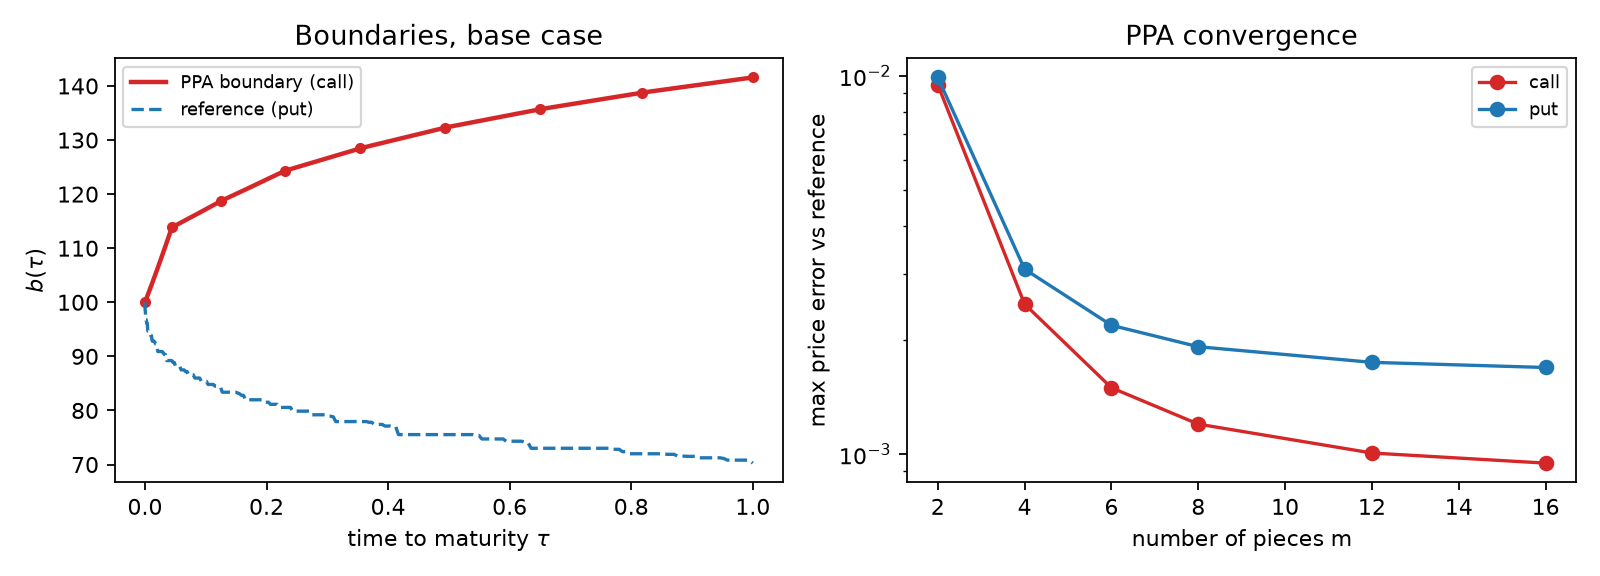
\includegraphics[keepaspectratio]{figures/f02_ppa.png}}

}

\caption{\label{fig-ppa}Left: PPA boundary (call, knots marked) against
the reference put boundary, base case. Right: error vs \(m\).}

\end{figure}%

\begin{figure}[tbp]

\centering{

\pandocbounded{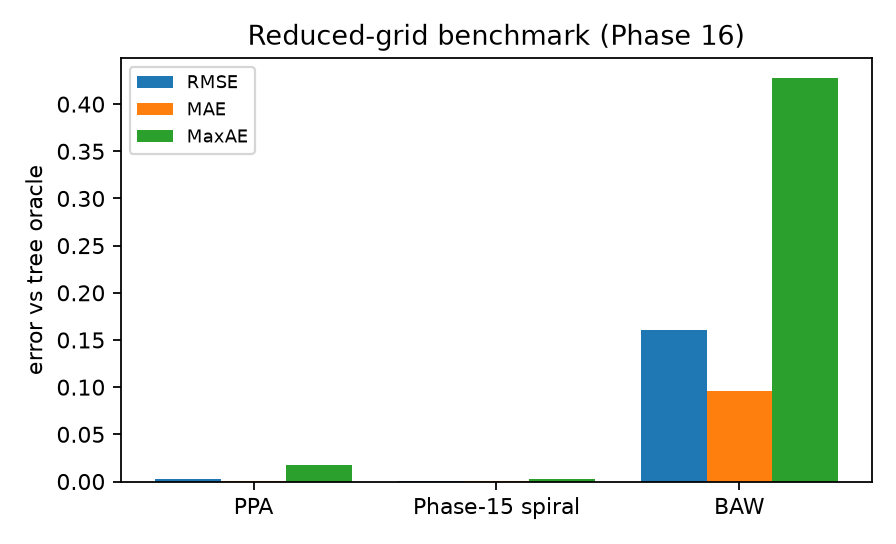
\includegraphics[keepaspectratio]{figures/f03_benchmark.png}}

}

\caption{\label{fig-benchmark}RMSE/MAE/MaxAE against the tree oracle on
the reduced grid.}

\end{figure}%

\subsection{Extended grid}\label{sec-extended}

\begin{longtable}[]{@{}llll@{}}
\caption{Extended 90-configuration benchmark against the converged tree
oracle (N=8000).}\label{tbl-extended}\tabularnewline
\toprule\noalign{}
Method & RMSE & MAE (mean) & MaxAE \\
\midrule\noalign{}
\endfirsthead
\toprule\noalign{}
Method & RMSE & MAE (mean) & MaxAE \\
\midrule\noalign{}
\endhead
\bottomrule\noalign{}
\endlastfoot
PPA (\(m=10\), pinned) & 0.0146 & 0.0026 & 0.212 \\
Phase 15 spiral (revised) & 0.0017 & 0.0010 & 0.008 \\
Barone-Adesi--Whaley & 0.2789 & 0.1620 & 1.131 \\
\end{longtable}

\section{Structural finding: the perpetual approach is not
exponential}\label{sec-decay}

Fit \(\ln|b(\tau)-b_\infty|=c-\kappa_{\mathrm{eff}}\tau\) on
successively later windows of the \(T=16\) reference solutions
(Figure~\ref{fig-decay}):

\begin{longtable}[]{@{}llll@{}}
\caption{Effective decay rates of \(|b(\tau)-b_\infty|\) by observation
window.}\label{tbl-rates}\tabularnewline
\toprule\noalign{}
Case & \([2,16]\) & \([6,16]\) & \([10,16]\) \\
\midrule\noalign{}
\endfirsthead
\toprule\noalign{}
Case & \([2,16]\) & \([6,16]\) & \([10,16]\) \\
\midrule\noalign{}
\endhead
\bottomrule\noalign{}
\endlastfoot
put, \(r=q=0.05\) & 0.142 & 0.120 & 0.101 \\
put, \(r=0.07,q=0.03\) & 0.169 & 0.130 & 0.169 \\
\end{longtable}

The rates \emph{drift} with the window: there is no single exponential.
The mechanism is visible in the linearization of the value-matching
equation around the perpetual solution: with
\(b(\tau)=b_\infty e^{\varepsilon(\tau)}\) and the exponential ansatz
\(\varepsilon=Ce^{-\kappa\tau}\), the kernel that carries boundary
memory, \(\partial f/\partial B\) at \((b_\infty,b_\infty)\), is
proportional to \((r-q)\) (the \(\Phi\)-parts cancel by the
Black--Scholes delta identity), so at \(r=q\) the characteristic
equation loses its \(\kappa\)-dependence entirely --- the memory enters
at higher order and the approach is slower than any rate the first-order
theory can name (consistent with the drifting fits). The practical
consequence is the design decision of Section~\ref{sec-ppa}: \textbf{pin
the boundary at the known perpetual limit instead of extrapolating a
decay law}.

\begin{figure}[tbp]

\centering{

\pandocbounded{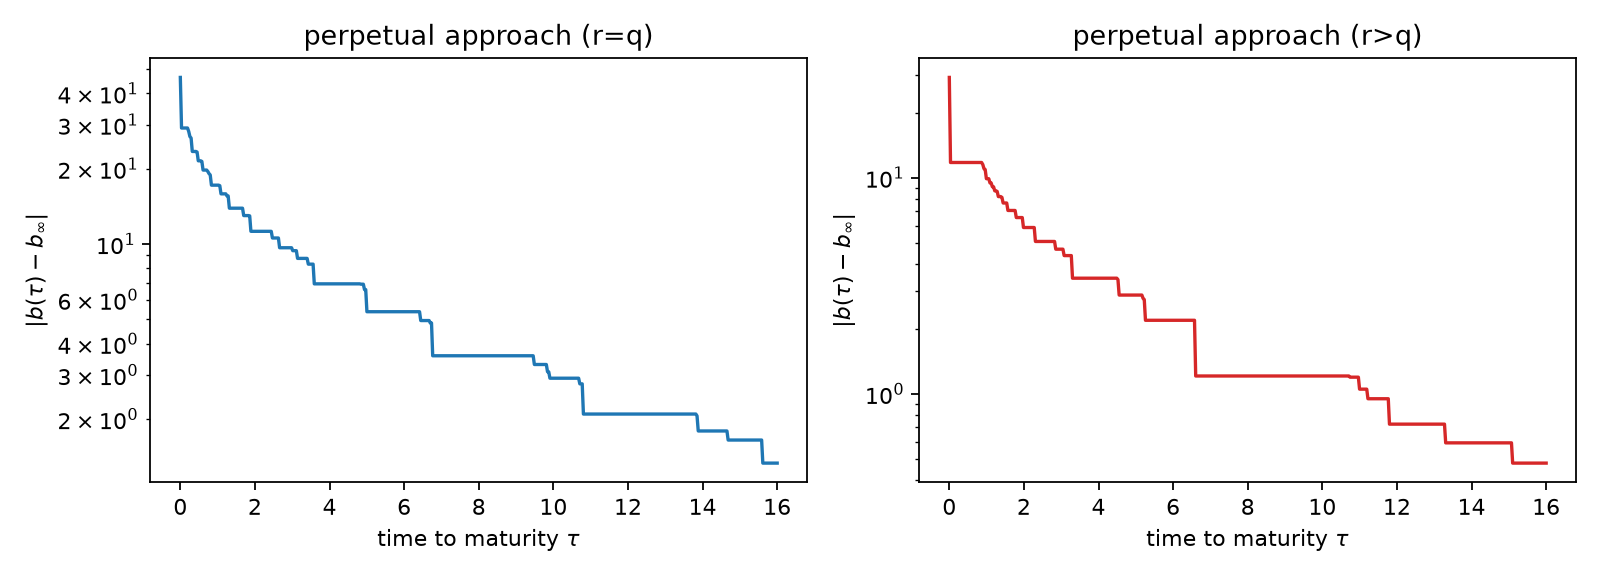
\includegraphics[keepaspectratio]{figures/f04_decay.png}}

}

\caption{\label{fig-decay}Absolute distance \(|b(\tau)-b_\infty|\) for
the put at \(r=q=0.05\) (left) and \(r=0.07,q=0.03\) (right), log scale;
the curvature shows the drift of effective rates.}

\end{figure}%

\section{Tier B probe: eliminating the collocation
solves}\label{sec-tierb}

A fully evaluation-only formula would replace the \(m\) collocation
solves by explicit surfaces \(\kappa_i(r,q,\sigma,T)\) (Phase 15 spiral
parameters) or knot-value surfaces. A 13-term quadratic feature fit
\((1,\sigma,r-q,T,\sigma^2,(r-q)^2,T^2,\sigma T,(r-q)T,\sigma(r-q),
\sigma^2 T,\sigma T^2,(r-q)\sigma T)\) of the collocated spiral
parameters on the reduced grid yields parameter RMS errors
\(0.08\)--\(0.33\) (\(\kappa_2\) worst), and end-to-end the
surface-driven price degrades from RMSE \(\approx0.009\) (collocated) to
\(\approx0.05\) --- an order above the collocated formula, though still
\(\sim3\times\) better than BAW. Likely remedies (\(T\)-band
partitioning, rational bases, direct knot-fraction fits) were probed
without crossing the threshold; the direction is documented as open. The
operative recipe remains Tier A: \(m\) scalar collocations (\(\sim0.07\)
s), zero integration.

\section{Scope and limitations}\label{sec-scope}

\begin{itemize}
\tightlist
\item
  \textbf{No closed form for the true boundary is claimed.} The
  free-boundary problem remains open; Eq.~\ref{eq-ppa} is closed-form
  \emph{given the piecewise phase-affine boundary}, whose knots are
  numerical (Tier A) --- honest positioning, not a claim of solution.
\item
  \textbf{No hidden clipping.} PPA prices are the raw European +
  closed-form EEP values; with approximate knots they can sit slightly
  outside no-arbitrage bounds, and those deviations are visible in the
  CSVs as diagnostic information rather than projected away. The bounds
  \(C_A\le S\), \(P_A\le K\) are not enforced by the formula.
\item
  \textbf{The Volterra solver is not the oracle.} Its grid sensitivity
  and flat-step fallbacks are documented in the Phase 15 revision; every
  number in this paper is measured against the converged
  Broadie--Detemple adjacent-averaged tree (spread reported per row).
\item
  \textbf{Environment sensitivity.} Long-maturity prices also drift at
  the \(10^{-2}\) scale with environment-level floating-point
  differences (e.g.~numpy SIMD paths); all paper numbers come from one
  environment (\texttt{phase3-paper}).
\item
  \textbf{Tier A is not evaluation-only.} The \(m\) scalar root-finds
  are fast but numerical; Tier B (explicit surfaces) is open
  (Section~\ref{sec-tierb}).
\item
  \textbf{Model scope.} Constant \(r,q,\sigma\), continuous dividends,
  standard single-asset American calls/puts.
\end{itemize}

\section{Reproducibility}\label{sec-repro}

All computations run in the existing \texttt{phase3-paper} conda
environment (Python 3.12, numpy 2.5.1, scipy 1.18.0, matplotlib 3.11.1);
no packages installed. Fixed seed \texttt{20260903}. Artifacts:

\begin{itemize}
\tightlist
\item
  \texttt{phase16\_closedform.py} --- occupation resolvent,
  affine/multipiece closed-form EEP, sequential collocation, perpetual
  pinning, adaptive knot insertion;
\item
  \texttt{tests/test\_phase16\_closedform.py} --- 12 tests; full suite
  218/218 green;
\item
  \texttt{notebooks/build\_phase16\_closedform.py} → executed
  \texttt{notebooks/phase16\_closedform.ipynb} --- the computational
  record behind every number above (figures \texttt{phase16\_figures/},
  tables \texttt{phase16\_tables/}, extended benchmark CSV);
\item
  \texttt{paper/phase16/} --- this manuscript, executed notebook copy,
  tables.
\end{itemize}

The notebook executes top-to-bottom from a clean kernel in under one
minute.

\section*{References}\label{references}
\addcontentsline{toc}{section}{References}

\protect\phantomsection\label{refs}
\begin{CSLReferences}{1}{1}
\bibitem[\citeproctext]{ref-carrjarrowmyneni1992}
Carr, Peter, Robert Jarrow, and Ravi Myneni. 1992. {``Alternative
Characterizations of {A}merican Put Options.''} \emph{Mathematical
Finance} 2 (2): 87--106.

\bibitem[\citeproctext]{ref-phase15paper}
Complex--Itô Random-Walk Research Project. 2026a. \emph{American Calls
and Puts Under {B}lack--{S}choles--{M}erton from One-Driver Complex
Geometric Brownian Motion}.

\bibitem[\citeproctext]{ref-phase4paper}
Complex--Itô Random-Walk Research Project. 2026b. \emph{Native Complex
Geometric Brownian Motion: Itô Correction, Stochastic Rotation, and
Noise-Dimension Geometry}.

\bibitem[\citeproctext]{ref-jacka1991}
Jacka, Saul D. 1991. {``Optimal Stopping and the {A}merican Put
Price.''} \emph{Annals of Applied Probability} 1 (1): 1--21.

\bibitem[\citeproctext]{ref-ju1998}
Ju, Nengjiu. 1998. {``Pricing an {A}merican Option by Approximating Its
Early Exercise Boundary as a Multipiece Exponential Function.''}
\emph{Review of Financial Studies} 11 (3): 627--46.

\bibitem[\citeproctext]{ref-kim1990}
Kim, In Joon. 1990. {``The Analytic Valuation of American Options.''}
\emph{Review of Financial Studies} 3 (4): 547--72.

\end{CSLReferences}




\end{document}
